% Provenance (never printed): 6e geography and cycle 3 sciences (locating a
% place on the globe: parallels, meridians, latitude, longitude; the Earth's
% rotation and time zones); see sources/book1/PROVENANCE.md.
% Book 1, grade 6, chapter 2.
\chapter{العرض والطول والمناطق الزمنية}\label{ch:g6:latitude-longitude}

حلّ الليل على \omterm{def:g2:water-on-earth:ocean}{المحيط}. على سطح سفينة شراعية، في عام
1750، يرفع الملّاح أداته نحو نجم لامع ويقيس
ارتفاعه فوق \omterm{def:g2:water-on-earth:ocean}{البحر}. دقائق قليلة من العمل، فيعرف كم
تبعد السفينة شمال \omterm{def:g3:continents-and-oceans:equator}{خط الاستواء}. لكن كم تبعد شرقًا أو غربًا؟ ذلك ما لا
يستطيع معرفته. وكانت المشكلة خطيرة إلى حد أن البرلمان البريطاني وعد عام 1714
بجائزة كبيرة لمن يجد طريقة لقياسه في \omterm{def:g2:water-on-earth:ocean}{البحر}.
واليوم، يعطيك الهاتف الذي في جيبك الجوابين في ثانية واحدة.
% ledger: rmg:15deg-per-hour, rmg:longitude-act-1714

\begin{omfigure}
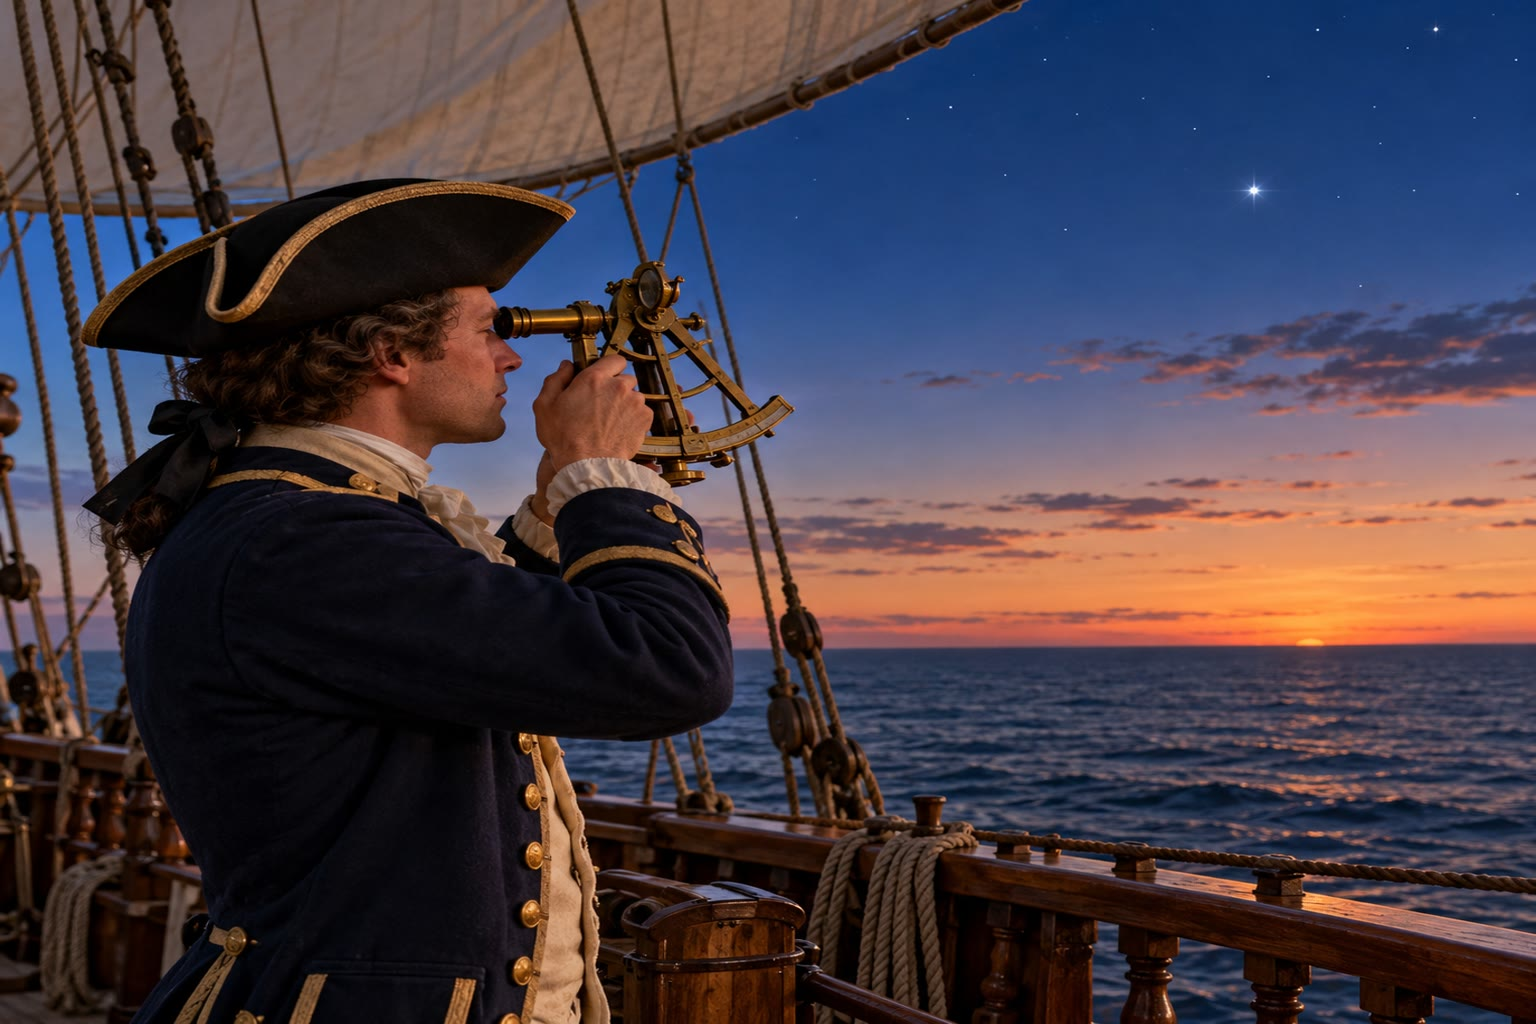
\includegraphics[width=0.62\linewidth]{images/book1/ai/g6-navigator-sextant.jpg}

{\small ملّاح من القرن الثامن عشر يقيس ارتفاع
نجم فوق أفق \omterm{def:g2:water-on-earth:ocean}{البحر}. (رسم بالذكاء الاصطناعي.)}
\end{omfigure}

\begin{recall}
\omterm{def:g3:continents-and-oceans:globe}{مجسم الكرة الأرضية} نموذج صغير للأرض. \omterm{def:g3:continents-and-oceans:equator}{وخط الاستواء} هو الخط الذي يدور
حول وسط \omterm{def:g3:continents-and-oceans:globe}{المجسم}، في منتصف المسافة بين \omterm{def:g3:continents-and-oceans:poles}{القطب الشمالي} \omterm{def:g3:continents-and-oceans:poles}{والقطب
الجنوبي}؛ وهو يقسم الأرض إلى \omterm{def:g3:continents-and-oceans:equator}{نصف الكرة الشمالي} \omterm{def:g3:continents-and-oceans:equator}{ونصف الكرة
الجنوبي} (\cref{ch:g3:continents-and-oceans}). وقد بيّنت كتب الفيزياء
أن الأرض تدور حول نفسها حول محور يمر \omterm{def:g3:continents-and-oceans:poles}{بالقطبين}، مرة
في اليوم: وهذا الدوران يأتي بالليل والنهار.
\end{recall}

\section{دوائر العرض والعرض الجغرافي}

لنقول أين يقع مكان على الأرض، نحتاج إلى عددين، مثل الصف
والعمود لمقعد في قاعة سينما. الأول يخبرنا كم يبعد المكان شمال
\omterm{def:g3:continents-and-oceans:equator}{خط الاستواء} أو جنوبه.

تخيّل الأرض مقطوعة نصفين، عبر \omterm{def:g3:continents-and-oceans:poles}{القطبين}، كتفاحة مقطوعة من
العنق نزولًا. على وجه القطع (إلى اليمين، أدناه)، \omterm{def:g3:continents-and-oceans:equator}{خط الاستواء} هو
الخط الأفقي المار بالمركز. والمكان~P على السطح يُرى من
المركز بزاوية معيّنة فوق ذلك الخط أو تحته: هذه الزاوية هي
عرضه الجغرافي.

\begin{omfigure}
\begin{minipage}[t]{0.48\linewidth}\centering
\begin{tikzpicture}[scale=0.95]
  \def\R{2.2}
  \fill[blue!6] (0,0) circle (\R);
  \draw[thick] (0,0) circle (\R);
  % parallels seen edge-on: horizontal chords
  \foreach \a in {-60,-30,30,60}{
    \draw[blue!45, densely dashed] ({-\R*cos(\a)},{\R*sin(\a)}) -- ({\R*cos(\a)},{\R*sin(\a)});}
    \draw[green!50!black, thick] (-\R,0) -- (\R,0);
  \node[font=\scriptsize, green!50!black, anchor=west] at (\R,0) {\foreignlanguage{arabic}{خط الاستواء $0^\circ$}};
  \draw[blue!60!black, thick] ({-\R*cos(40)},{\R*sin(40)}) -- ({\R*cos(40)},{\R*sin(40)});
  \draw[->, thick] (0,0) -- ({\R*cos(40)},{\R*sin(40)});
  \fill (0,0) circle (1.4pt) node[below left, font=\scriptsize, inner sep=1pt] {المركز};
  \fill ({\R*cos(40)},{\R*sin(40)}) circle (1.6pt)
    node[above right, font=\scriptsize\bfseries, inner sep=1pt] {P};
  \draw[red!70!black, thick] (0.9,0) arc (0:40:0.9);
  \node[red!70!black, font=\scriptsize] at (20:1.25) {$40^\circ$};
  \node[font=\scriptsize, blue!60!black, anchor=east] at ({-\R*cos(40)},{\R*sin(40)}) {\foreignlanguage{arabic}{دائرة العرض $40^\circ$ ش}};
  \fill (0,\R) circle (1.4pt) node[above, font=\scriptsize] {\foreignlanguage{arabic}{القطب الشمالي $90^\circ$ ش}};
  \fill (0,-\R) circle (1.4pt) node[below, font=\scriptsize] {\foreignlanguage{arabic}{القطب الجنوبي $90^\circ$ ج}};
\end{tikzpicture}

{\small \omterm{def:g6:latitude-longitude:latitude}{العرض الجغرافي}: الزاوية عند مركز الأرض بين \omterm{def:g3:continents-and-oceans:equator}{خط الاستواء}
والمكان.}
\end{minipage}\hfill
\begin{minipage}[t]{0.48\linewidth}\centering
\begin{tikzpicture}[scale=0.95]
  \def\R{2.2}
  \fill[green!6] (0,0) circle (\R);
  \draw[thick] (0,0) circle (\R);
  \foreach \a in {0,30,...,330}{\draw[black!25] (0,0) -- (\a:\R);}
    \draw[red!70!black, very thick] (0,0) -- (270:\R)
    node[below, font=\scriptsize, align=center] {خط الزوال الأصلي\\\foreignlanguage{arabic}{(غرينتش)، $0^\circ$}};
  \draw[blue!60!black, very thick] (0,0) -- (330:\R)
    node[right, font=\scriptsize] {\foreignlanguage{arabic}{$60^\circ$ ق}};
  \draw[black!60, thick] (0,0) -- (210:\R) node[left, font=\scriptsize] {\foreignlanguage{arabic}{$60^\circ$ غ}};
  \draw[black!60, thick] (0,0) -- (90:\R) node[above, font=\scriptsize] {$180^\circ$};
  \draw[red!70!black, thick] (270:0.9) arc (270:330:0.9);
  \node[red!70!black, font=\scriptsize] at (300:1.25) {$60^\circ$};
    \fill (0,0) circle (1.6pt) node[above left, font=\scriptsize, inner sep=1.5pt, fill=green!6] {القطب الشمالي};
  \draw[->, thick, black!70] (40:2.55) arc (40:80:2.55);
  \node[font=\scriptsize, black!70, anchor=south west] at (55:2.6) {الأرض تدور};
  \node[font=\scriptsize, anchor=west] at (2.0,-1.6) {\foreignlanguage{arabic}{الشرق $\circlearrowleft$}};
\end{tikzpicture}

{\small \omterm{def:g6:latitude-longitude:longitude}{الطول الجغرافي}: الأرض كما تُرى من فوق \omterm{def:g3:continents-and-oceans:poles}{القطب الشمالي}. تُقاس الزاوية
من \omterm{def:g6:latitude-longitude:longitude}{خط الزوال الأصلي}، نحو الشرق أو نحو الغرب.}
\end{minipage}
% ledger: rmg:latitude-def, rmg:longitude-def
\end{omfigure}

\begin{definition}[دائرة العرض والعرض الجغرافي]\label{def:g6:latitude-longitude:latitude}
\emph{دائرة العرض}\index{دائرة العرض} دائرة مرسومة حول \omterm{def:g3:continents-and-oceans:globe}{المجسم} موازية
\omterm{def:g3:continents-and-oceans:equator}{لخط الاستواء}؛ وكل الأماكن الواقعة على دائرة العرض نفسها على البعد نفسه
من \omterm{def:g3:continents-and-oceans:equator}{خط الاستواء}. و\emph{العرض الجغرافي}\index{عرض جغرافي} لمكان ما هو الزاوية،
المقيسة عند مركز الأرض، بين \omterm{def:g3:continents-and-oceans:equator}{خط الاستواء} وذلك المكان. ويمتد
من $0^\circ$ عند \omterm{def:g3:continents-and-oceans:equator}{خط الاستواء} إلى $90^\circ$ عند \omterm{def:g3:continents-and-oceans:poles}{القطبين}، ونذكر
هل يقع المكان شمال \omterm{def:g3:continents-and-oceans:equator}{خط الاستواء} (ش) أم جنوبه (ج).
% ledger: rmg:latitude-def
\end{definition}

\omterm{def:g3:continents-and-oceans:equator}{خط الاستواء} نفسه دائرة عرض، وهو أطولها، وعرضه $0^\circ$.
وتقصر \omterm{def:g6:latitude-longitude:latitude}{دوائر العرض} كلما اقتربنا من \omterm{def:g3:continents-and-oceans:poles}{القطبين}، وكل \omterm{def:g3:continents-and-oceans:poles}{قطب} نقطة
واحدة، عند $90^\circ$ شمالًا أو $90^\circ$ جنوبًا. وعلى طول خط يمتد من \omterm{def:g3:continents-and-oceans:poles}{قطب} إلى
\omterm{def:g3:continents-and-oceans:equator}{خط الاستواء}، تقيس كل درجة من \omterm{def:g6:latitude-longitude:latitude}{درجات العرض} نحو \qty{111}{km}.
% ledger: rmg:latitude-def

\omterm{def:g6:latitude-longitude:latitude}{العرض الجغرافي} هو العدد السهل: يمكن إيجاده من السماء. ففي النهار،
كان البحارة يقيسون ارتفاع الشمس عند الظهر؛ وفي الليل، في \omterm{def:g3:continents-and-oceans:equator}{نصف الكرة
الشمالي}، كانوا يقيسون ارتفاع النجم القطبي. وهذا ما يفعله
ملّاح الصورة في أول الفصل.
% ledger: rmg:15deg-per-hour

يقع النجم القطبي تقريبًا على امتداد محور الأرض تمامًا،
وراء \omterm{def:g3:continents-and-oceans:poles}{القطب الشمالي}، وهو بعيد إلى حد أن ضوءه يصل إلى
كل مكان على الأرض في خطوط متوازية. وعند \omterm{def:g3:continents-and-oceans:poles}{القطب الشمالي} يكون
فوق الرأس تمامًا، على ارتفاع $90^\circ$ فوق الأفق؛ وعند \omterm{def:g3:continents-and-oceans:equator}{خط الاستواء} يقع
على الأفق الشمالي، عند $0^\circ$. وبين ذلك، القاعدة بسيطة:
\emph{ارتفاع النجم القطبي فوق الأفق الشمالي، مقيسًا
بزاوية، يساوي \omterm{def:g6:latitude-longitude:latitude}{العرض الجغرافي}}. والشكل أدناه يبين لماذا كانت
الزاويتان متساويتين.
% ledger: nsta:polaris-latitude

\begin{omfigure}
\begin{tikzpicture}[scale=1.1, font=\scriptsize]
  \def\R{1.7}
  \coordinate (O) at (0,0);
  \coordinate (P) at ({\R*cos(40)},{\R*sin(40)});
  \fill[blue!8] (O) circle (\R);
  \draw[black!70] (O) circle (\R);
  % equator and axis
  \draw[black!50] (-\R,0) -- (\R,0);
  \node[black!60, anchor=north east] at (-0.15,0) {خط الاستواء};
  \draw[black!70, -{Stealth[length=2mm]}] (0,-\R-0.3) -- (0,\R+1.7);
  \node[anchor=east, align=right] at (-0.1,\R+1.45) {نحو النجم القطبي\\\foreignlanguage{arabic}{(بعيد جدًا)}};
  \node[anchor=south east] at (0,\R) {ش};
  % radius to P and latitude angle at the centre
  \draw[black!80] (O) -- (P);
  \draw[red!70!black, thick] (0.55,0) arc (0:40:0.55);
  \node[red!70!black] at (20:0.8) {$40^\circ$};
  % horizon at P (tangent) and the ray to the Pole Star (parallel to the axis)
  \draw[black!70, thick] ($(P)+({-sin(40)*1.5},{cos(40)*1.5})$) -- ($(P)+({sin(40)*1.6},{-cos(40)*1.6})$);
  \node[anchor=south, rotate=-50, inner sep=2pt] at ($(P)+({sin(40)*1.15},{-cos(40)*1.15})$) {الأفق};
  \draw[orange!80!black, thick, -{Stealth[length=2mm]}] (P) -- ++(0,1.45);
  \draw[red!70!black, thick] ($(P)+(0,0.7)$) arc (90:130:0.7);
  \node[red!70!black] at ($(P)+(110:0.98)$) {$40^\circ$};
  \fill (P) circle (1.4pt);
  \node[anchor=west] at ($(P)+(0.3,0.05)$) {\foreignlanguage{arabic}{راصد عند $40^\circ$ ش}};
\end{tikzpicture}

{\small لماذا يساوي ارتفاع النجم القطبي \omterm{def:g6:latitude-longitude:latitude}{العرض الجغرافي} (رسم تخطيطي، دون
مراعاة النسب). ضوء النجم القطبي يصل موازيًا لمحور الأرض
(بالبرتقالي). وأفق الراصد عمودي على نصف القطر
المار بالراصد؛ والمحور عمودي على \omterm{def:g3:continents-and-oceans:equator}{خط الاستواء}. لذلك فالزاوية
بين الأفق والنجم القطبي تساوي \omterm{def:g6:latitude-longitude:latitude}{العرض الجغرافي}، أي
الزاوية عند المركز بين \omterm{def:g3:continents-and-oceans:equator}{خط الاستواء} والراصد.}
% ledger: nsta:polaris-latitude
\end{omfigure}

\begin{example}[ملّاحة في الليل]\label{ex:g6:latitude-longitude:pole-star}
تقيس ملّاحة ارتفاع النجم القطبي فتجده $41^\circ$ فوق الأفق
الشمالي. فالسفينة على \omterm{def:g6:latitude-longitude:latitude}{العرض} $41^\circ$ شمالًا، أي على نحو $41 \times 111
\approx \num{4550}$~km شمال \omterm{def:g3:continents-and-oceans:equator}{خط الاستواء}. وإذا أبحرت شمالًا، وجدت
النجم أعلى قليلًا كل ليلة؛ وإذا أبحرت جنوبًا نحو \omterm{def:g3:continents-and-oceans:equator}{خط الاستواء}،
هبط نحو الأفق. وجنوب \omterm{def:g3:continents-and-oceans:equator}{خط الاستواء} لا يمكن رؤية النجم القطبي
أبدًا، لأنه يبقى تحت الأفق: وهناك، تعطي شمس الظهر
\omterm{def:g6:latitude-longitude:latitude}{العرض الجغرافي}.
\end{example}
% ledger: nsta:polaris-latitude, rmg:latitude-def, rmg:15deg-per-hour

\section{خطوط الزوال والطول الجغرافي}

العدد الثاني يخبرنا كم يبعد المكان شرقًا أو غربًا. وهنا لا يوجد
خط بداية طبيعي مثل \omterm{def:g3:continents-and-oceans:equator}{خط الاستواء}: فلا بد من اختيار واحد.

\begin{definition}[خط الزوال والطول الجغرافي وخط الزوال الأصلي]\label{def:g6:latitude-longitude:longitude}
\emph{خط الزوال}\index{خط الزوال} نصف دائرة مرسوم على \omterm{def:g3:continents-and-oceans:globe}{المجسم} من
\omterm{def:g3:continents-and-oceans:poles}{القطب الشمالي} إلى \omterm{def:g3:continents-and-oceans:poles}{القطب الجنوبي}. و\emph{خط الزوال الأصلي}\index{خط الزوال الأصلي}
هو خط الزوال الذي اختير خطَّ بداية: الخط المار
بالمرصد الملكي القديم في غرينتش، في لندن.
و\emph{الطول الجغرافي}\index{طول جغرافي} لمكان ما هو الزاوية بين خط الزوال
الأصلي وخط زوال ذلك المكان، كما تُرى من محور الأرض. ويمتد
من $0^\circ$ عند خط الزوال الأصلي إلى $180^\circ$، ونذكر هل
يقع المكان شرق خط الزوال الأصلي (ق) أم غربه (غ).
% ledger: rmg:longitude-def
\end{definition}

تلتقي \omterm{def:g6:latitude-longitude:longitude}{خطوط الزوال} كلها عند \omterm{def:g3:continents-and-oceans:poles}{القطبين}، وكلها بالطول نفسه. وفي
الجهة المقابلة من الأرض لغرينتش، يكون \omterm{def:g6:latitude-longitude:longitude}{خط الزوال} $180^\circ$ شرقًا
\omterm{def:g6:latitude-longitude:longitude}{وخط الزوال} $180^\circ$ غربًا الخطَّ نفسه.

\begin{omfigure}
\begin{minipage}[c]{0.46\linewidth}\centering
\begin{tikzpicture}
  \begin{axis}[axis equal image, hide axis, width=\linewidth,
      xmin=-1.05, xmax=1.05, ymin=-1.05, ymax=1.12, clip=false]
    \fill[omSea] (axis cs:0,0) circle (1);
    \addplot[fill=omLithAlluv, draw=black!45, line width=0.2pt] table {figdata/out/grade-6-graticule-land.dat};
    \addplot[blue!50!black, line width=0.35pt] table {figdata/out/grade-6-graticule-parallels.dat};
    \addplot[black!55, line width=0.35pt] table {figdata/out/grade-6-graticule-meridians.dat};
        \addplot[green!50!black, line width=1.1pt] table {figdata/out/grade-6-graticule-equator.dat};
    \addplot[red!70!black, line width=1.1pt] table {figdata/out/grade-6-graticule-prime.dat};
    \draw[black!70] (axis cs:0,0) circle (1);
    \fill (axis cs:0,0.9063) circle (1.3pt);
        \node[font=\scriptsize, above left, inner sep=1.5pt] at (axis cs:0,0.9063) {ش};
  \end{axis}
\end{tikzpicture}
\end{minipage}\hfill
\begin{minipage}[c]{0.5\linewidth}
{\small \omterm{def:g3:continents-and-oceans:globe}{مجسم كرة أرضية} بدوائر عرضه (بالأزرق) وخطوط زواله (بالرمادي)، كل
$30^\circ$. \omterm{def:g3:continents-and-oceans:equator}{خط الاستواء} مرسوم بالأخضر السميك، \omterm{def:g6:latitude-longitude:longitude}{وخط الزوال الأصلي}
بالأحمر؛ ويتقاطعان في \omterm{def:g2:water-on-earth:ocean}{المحيط} جنوب غانا، عند \omterm{def:g6:latitude-longitude:latitude}{العرض} $0^\circ$،
\omterm{def:g6:latitude-longitude:longitude}{والطول} $0^\circ$. كل خط زوال يمتد من \omterm{def:g3:continents-and-oceans:poles}{قطب} إلى \omterm{def:g3:continents-and-oceans:poles}{قطب}؛ وكل دائرة عرض
دائرة حول المحور. (اليابسة: Natural Earth.)}
% ledger: data:ne-land (figdata/grade-6/graticule.py)
\end{minipage}
\end{omfigure}

\begin{history}[اختيار خط الزوال الأصلي]
زمنًا طويلًا، كان كل بلد يرسم خرائطه بخط زوال بداية خاص به:
فاستُعملت لندن وباريس وأماكن أخرى. وفي أكتوبر 1884، اجتمع مندوبو
بلدان كثيرة في واشنطن لاختيار خط زوال واحد للعالم كله.
وفي 13~أكتوبر، صوّتوا على اقتراح \omterm{def:g6:latitude-longitude:longitude}{خط الزوال} المار
بمرصد غرينتش: فصوّت له 21 بلدًا، وعارضه بلد واحد، وامتنع
بلدان عن التصويت.
% ledger: rmg:longitude-def, meridian:1884-vote
\end{history}

\section{إيجاد مكان بزاويتيه}

\omterm{def:g6:latitude-longitude:latitude}{بالعرض} \omterm{def:g6:latitude-longitude:longitude}{والطول} الجغرافيين، يمكن إيجاد أي مكان على الأرض،
على \omterm{def:g2:drawing-to-map:map}{خريطة} أو على \omterm{def:g3:continents-and-oceans:globe}{مجسم}. ونكتب \omterm{def:g6:latitude-longitude:latitude}{العرض} أولًا: فالقاهرة، مثلًا،
تقع على نحو $30^\circ$ شمالًا، $31^\circ$ شرقًا.
% ledger: data:b1-ne-places (figdata/grade-6/cities.py)

\begin{omfigure}
\begin{tikzpicture}
  \begin{axis}[ommap, width=\linewidth,
      xtick={-180,-150,...,180}, ytick={-90,-60,...,90},
      xticklabels={$180^\circ$,\foreignlanguage{arabic}{$150^\circ$ غ},\foreignlanguage{arabic}{$120^\circ$ غ},\foreignlanguage{arabic}{$90^\circ$ غ},\foreignlanguage{arabic}{$60^\circ$ غ},\foreignlanguage{arabic}{$30^\circ$ غ},$0^\circ$,
                   \foreignlanguage{arabic}{$30^\circ$ ق},\foreignlanguage{arabic}{$60^\circ$ ق},\foreignlanguage{arabic}{$90^\circ$ ق},\foreignlanguage{arabic}{$120^\circ$ ق},\foreignlanguage{arabic}{$150^\circ$ ق},$180^\circ$},
      yticklabels={\foreignlanguage{arabic}{$90^\circ$ ج},\foreignlanguage{arabic}{$60^\circ$ ج},\foreignlanguage{arabic}{$30^\circ$ ج},$0^\circ$,\foreignlanguage{arabic}{$30^\circ$ ش},\foreignlanguage{arabic}{$60^\circ$ ش},\foreignlanguage{arabic}{$90^\circ$ ش}},
      tick label style={font=\tiny}, grid style={black!35, line width=0.3pt}]
    \addplot[fill=omLithAlluv, draw=black!45, line width=0.2pt] table {figdata/out/shared-geo-land.dat};
        \draw[green!50!black, line width=0.9pt] (axis cs:-180,0) -- (axis cs:180,0);
    \draw[red!70!black, line width=0.9pt] (axis cs:0,-90) -- (axis cs:0,90);
    \addplot[only marks, mark=*, mark size=1.2pt, black]
      table[x=lon, y=lat] {figdata/out/grade-6-cities-map.dat};
    \node[font=\tiny, inner sep=1.2pt, fill=white, fill opacity=0.75, text opacity=1, anchor=south] at (axis cs:-21.936,64.144) {ريكيافيك};
    \node[font=\tiny, inner sep=1.2pt, fill=white, fill opacity=0.75, text opacity=1, anchor=south] at (axis cs:-0.119,51.502) {لندن};
    \node[font=\tiny, inner sep=1.2pt, fill=white, fill opacity=0.75, text opacity=1, anchor=west] at (axis cs:-73.996,40.722) {نيويورك};
    \node[font=\tiny, inner sep=1.2pt, fill=white, fill opacity=0.75, text opacity=1, anchor=east] at (axis cs:-118.232,34.049) {لوس أنجلوس};
    \node[font=\tiny, inner sep=1.2pt, fill=white, fill opacity=0.75, text opacity=1, anchor=east] at (axis cs:-78.502,-0.213) {كيتو};
    \node[font=\tiny, inner sep=1.2pt, fill=white, fill opacity=0.75, text opacity=1, anchor=west] at (axis cs:-43.212,-22.907) {ريو دي جانيرو};
    \node[font=\tiny, inner sep=1.2pt, fill=white, fill opacity=0.75, text opacity=1, anchor=north] at (axis cs:18.433,-33.918) {كيب تاون};
    \node[font=\tiny, inner sep=1.2pt, fill=white, fill opacity=0.75, text opacity=1, anchor=west] at (axis cs:36.815,-1.281) {نيروبي};
    \node[font=\tiny, inner sep=1.2pt, fill=white, fill opacity=0.75, text opacity=1, anchor=south] at (axis cs:31.248,30.052) {القاهرة};
    \node[font=\tiny, inner sep=1.2pt, fill=white, fill opacity=0.75, text opacity=1, anchor=north] at (axis cs:72.876,19.068) {مومباي};
    \node[font=\tiny, inner sep=1.2pt, fill=white, fill opacity=0.75, text opacity=1, anchor=west] at (axis cs:139.75,35.687) {طوكيو};
    \node[font=\tiny, inner sep=1.2pt, fill=white, fill opacity=0.75, text opacity=1, anchor=south] at (axis cs:151.213,-33.871) {سيدني};
    \node[font=\tiny, inner sep=1.2pt, fill=white, fill opacity=0.75, text opacity=1, anchor=north east] at (axis cs:174.763,-36.848) {أوكلاند};
  \end{axis}
\end{tikzpicture}

{\small ثلاث عشرة مدينة على \omterm{def:g3:continents-and-oceans:world-map}{خريطة للعالم} بشبكة كل $30^\circ$. \omterm{def:g3:continents-and-oceans:equator}{خط
الاستواء} مرسوم بالأخضر، \omterm{def:g6:latitude-longitude:longitude}{وخط الزوال الأصلي} بالأحمر. (\omterm{def:g1:landscapes-around-us:water}{السواحل}
والمدن: Natural Earth.)}
% ledger: data:ne-land, data:b1-ne-places (figdata/grade-6/cities.py, part map)
\end{omfigure}

\begin{method}[تحديد موقع مكان بإحداثياته]\label{met:g6:latitude-longitude:locating}
\begin{enumerate}
  \item \omterm{def:g6:latitude-longitude:latitude}{العرض الجغرافي}: انطلق من \omterm{def:g3:continents-and-oceans:equator}{خط الاستواء} واتجه شمالًا (ش) أو جنوبًا (ج)،
        عادًّا \omterm{def:g6:latitude-longitude:latitude}{دوائر العرض}، حتى العدد الصحيح من الدرجات.
  \item \omterm{def:g6:latitude-longitude:longitude}{الطول الجغرافي}: انطلق من \omterm{def:g6:latitude-longitude:longitude}{خط الزوال الأصلي} واتجه شرقًا (ق) أو غربًا
        (غ)، عادًّا \omterm{def:g6:latitude-longitude:longitude}{خطوط الزوال}، حتى العدد الصحيح من الدرجات.
  \item المكان حيث تتقاطع \omterm{def:g6:latitude-longitude:latitude}{دائرة العرض} \omterm{def:g6:latitude-longitude:longitude}{وخط الزوال}. وبين خطين
        من خطوط الشبكة، قدّر: منتصف المسافة بين $30^\circ$
        و$60^\circ$ هو $45^\circ$.
\end{enumerate}
\end{method}

\begin{example}[قراءة إحداثيات سيدني]\label{ex:g6:latitude-longitude:sydney}
على \omterm{def:g2:drawing-to-map:map}{الخريطة}، تقع سيدني تحت \omterm{def:g3:continents-and-oceans:equator}{خط الاستواء}: فهي في \omterm{def:g3:continents-and-oceans:equator}{نصف الكرة
الجنوبي}، فوق \omterm{def:g6:latitude-longitude:latitude}{دائرة العرض} $30^\circ$ جنوبًا بقليل، أقرب إلى $30^\circ$
منها إلى $60^\circ$؛ فعرضها نحو $34^\circ$ جنوبًا. وتقع إلى يمين
\omterm{def:g6:latitude-longitude:longitude}{خط الزوال الأصلي}، بعد \omterm{def:g6:latitude-longitude:longitude}{خط الزوال} $150^\circ$ شرقًا بقليل؛ فطولها
نحو $151^\circ$ شرقًا. ونكتب: سيدني، $34^\circ$ جنوبًا،
$151^\circ$ شرقًا.
% ledger: data:b1-ne-places (cities.py: 33.87 S, 151.21 E)
\end{example}

\section{الأرض الدوّارة والمناطق الزمنية}

تدور الأرض حول نفسها مرة في اليوم، من الغرب إلى الشرق. وبدورانها، تبدو
الشمس كأنها تعبر السماء من الشرق إلى الغرب. وحين تكون الشمس في أعلى نقطة
لها في السماء، يكون الظهر. لكن الظهر لا يكون في كل مكان في اللحظة نفسها:
فحين يكون الظهر في لندن، يكون قد حلّ بعد الظهر في القاهرة، الأبعد شرقًا،
ويكون ما زال الصباح في نيويورك، الأبعد غربًا.

كم تدور الأرض في ساعة واحدة؟ الدورة الكاملة $360^\circ$،
وتستغرق 24~ساعة:
\[
360^\circ \div 24 = 15^\circ \text{ في الساعة.}
\]
فالمكانان اللذان يفصل بينهما $15^\circ$ من \omterm{def:g6:latitude-longitude:longitude}{الطول} يفصل بين ظهريهما ساعة واحدة:
والمكان الأبعد شرقًا يبلغه أولًا. والدرجة الواحدة تستغرق 4~دقائق.
% ledger: planet:Earth.day, rmg:15deg-per-hour

\begin{definition}[المنطقة الزمنية]\label{def:g6:latitude-longitude:time-zone}
\emph{المنطقة الزمنية}\index{منطقة زمنية} شريط من الأرض، من \omterm{def:g3:continents-and-oceans:poles}{قطب} إلى
\omterm{def:g3:continents-and-oceans:poles}{قطب}، تُظهر فيه كل الساعات الوقت نفسه. ومثاليًا، يكون عرض كل منطقة
$15^\circ$ من \omterm{def:g6:latitude-longitude:longitude}{الطول}، فيكون هناك 24 منطقة، واحدة لكل
ساعة؛ وكلما انتقلنا منطقة واحدة نحو الشرق، أظهرت الساعات ساعة زائدة.
\end{definition}

في المناطق المثالية، منطقة المكان هي طوله مقسومًا على $15$،
مقرّبًا إلى أقرب عدد صحيح: شرق غرينتش نضيف ذلك العدد من
الساعات إلى الوقت في غرينتش، وغربه نطرحه. فطوكيو، عند
$140^\circ$ شرقًا: $140 \div 15 \approx 9.3$، فالمنطقة $+9$: فحين يكون
الظهر في غرينتش، تكون الساعة 9~مساءً في طوكيو. \omterm{def:g6:latitude-longitude:time-zone}{والمناطق الزمنية} الحقيقية ليست أشرطة
مستقيمة: فهي تتبع حدود البلدان والأقاليم، لكي يحافظ بلد كامل،
أو إقليم كامل، على الوقت نفسه.
% ledger: data:b1-ne-places, rmg:15deg-per-hour

\begin{omfigure}
\begin{tikzpicture}
  \begin{axis}[ommap, width=\linewidth, clip=false,
      xtick={-180,-90,0,90,180}, ytick={-60,0,60},
      xticklabels={$180^\circ$,\foreignlanguage{arabic}{$90^\circ$ غ},$0^\circ$,\foreignlanguage{arabic}{$90^\circ$ ق},$180^\circ$},
      yticklabels={\foreignlanguage{arabic}{$60^\circ$ ج},$0^\circ$,\foreignlanguage{arabic}{$60^\circ$ ش}},
      tick label style={font=\tiny}, grid=none]
    \addplot[fill=black!8, draw=none] table {figdata/out/grade-6-time_zones-odd.dat};
    \addplot[fill=omLithAlluv, fill opacity=0.85, draw=black!45, line width=0.2pt] table {figdata/out/shared-geo-land.dat};
    \addplot[only marks, mark=none, point meta=explicit symbolic,
        nodes near coords, nodes near coords style={font=\tiny, anchor=south, inner sep=1pt}]
            table[x=lon, y=y, meta=label] {figdata/out/grade-6-time_zones-labels.dat};
    \draw[red!75!black, line width=1.6pt] (axis cs:180,-90) -- (axis cs:180,90);
    \draw[red!75!black, line width=1.6pt] (axis cs:-180,-90) -- (axis cs:-180,90);
        \draw[black, line width=0.8pt] (axis cs:0,-90) -- (axis cs:0,90);
    \node[font=\scriptsize, red!75!black, rotate=90, anchor=south] at (axis cs:180,0) {خط التاريخ};
    \node[font=\scriptsize, red!75!black, rotate=90, anchor=north] at (axis cs:-180,0) {خط التاريخ};
  \end{axis}
\end{tikzpicture}

{\small \omterm{def:g6:latitude-longitude:time-zone}{المناطق الزمنية} المثالية الأربع والعشرون، عرض كل منها $15^\circ$، مع عدد
الساعات التي تُضاف إلى الوقت في غرينتش (الخط الأسود في الوسط). ويمتد \omterm{def:g6:latitude-longitude:date-line}{خط التاريخ}
على \omterm{def:g6:latitude-longitude:longitude}{خط الزوال} $180^\circ$، الذي تقطعه هذه \omterm{def:g2:drawing-to-map:map}{الخريطة} نصفين: فهو
الحافة اليسرى والحافة اليمنى معًا. لُفّ \omterm{def:g2:drawing-to-map:map}{الخريطة} أنبوبًا، يصر الخطان الأحمران
خطًا واحدًا. والمنطقة الواقعة على كل جانب من \omterm{def:g6:latitude-longitude:date-line}{خط التاريخ} عرضها نصف منطقة.}
% ledger: rmg:15deg-per-hour, planet:Earth.day (figdata/grade-6/time_zones.py)
\end{omfigure}

\paragraph{خط التاريخ.} سافر شرقًا من غرينتش، مضيفًا ساعة لكل
منطقة: عند $180^\circ$ تكون متقدمًا 12~ساعة. وسافر غربًا، طارحًا ساعة
لكل منطقة: عند $180^\circ$ تكون متأخرًا 12~ساعة. فيلتقي المسافران
على \omterm{def:g6:latitude-longitude:longitude}{خط الزوال} نفسه وساعتاهما تُظهران الساعة نفسها، لكن بينهما يوم
كامل! فلا بد لأحدهما من أن يغيّر التاريخ.

\begin{definition}[خط التاريخ الدولي]\label{def:g6:latitude-longitude:date-line}
\emph{خط التاريخ الدولي}\index{خط التاريخ الدولي} هو
الخط، في وسط \omterm{def:g2:water-on-earth:ocean}{المحيط} الهادئ، الذي يتغير عنده التاريخ. وهو يتبع
\omterm{def:g6:latitude-longitude:longitude}{خط الزوال} $180^\circ$، مع بعض الانعطافات لكي لا يقسم بلدًا نصفين.
فعند عبوره نحو الغرب، ننتقل إلى اليوم التالي؛ وعند عبوره نحو
الشرق، نعود إلى اليوم السابق.
\end{definition}

\begin{history}[ساعة هاريسون البحرية]
\begin{minipage}[c]{0.7\linewidth}
ليجد الملّاح طوله الجغرافي، يقارن بين وقتين: الوقت المحلي على
السفينة، المقروء من الشمس، والوقت في اللحظة نفسها في ميناء الوطن.
وكل ساعة من الفرق تعني $15^\circ$ من \omterm{def:g6:latitude-longitude:longitude}{الطول}. وكانت الصعوبة
في حمل وقت الوطن عبر \omterm{def:g2:water-on-earth:ocean}{المحيط}: فحتى أفضل ساعات ذلك الزمن
لم تكن دقيقة بما يكفي. وقد أمضى صانع الساعات الإنجليزي جون هاريسون عقودًا
في المسألة، طامحًا إلى ساعة لا تتقدم ولا تتأخر أكثر من
3~ثوانٍ في اليوم. وساعته البحرية الرابعة، المسماة H4، تشبه ساعة جيب
كبيرة وتدق خمس مرات في الثانية. وفي عام 1761، أخذها ابنه ويليام في
رحلة إلى جامايكا لاختبارها.
% ledger: rmg:15deg-per-hour, rmg:longitude-act-1714, rmg:h4-jamaica-1761
\end{minipage}\hfill
\begin{minipage}[c]{0.26\linewidth}\centering
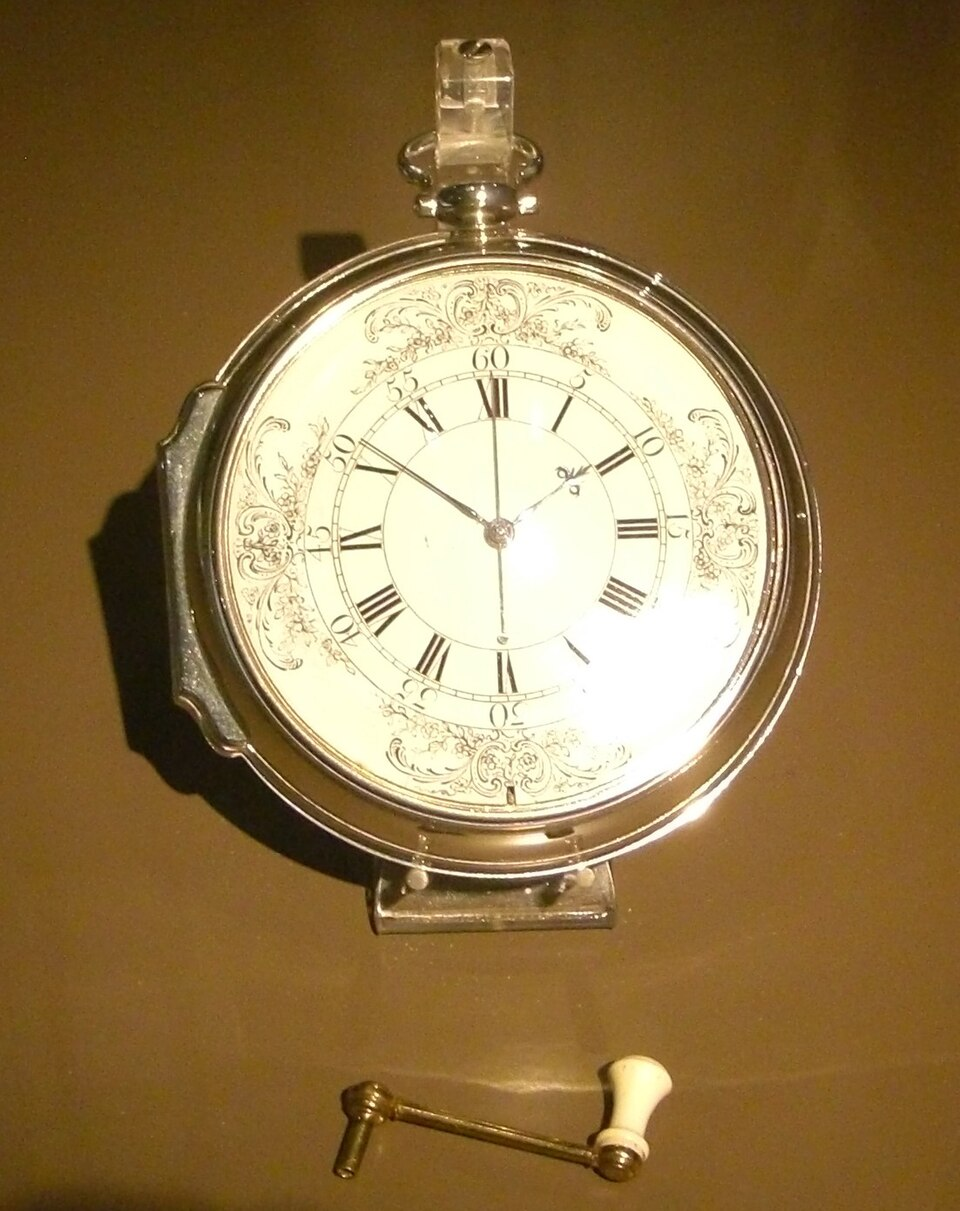
\includegraphics[width=\linewidth]{images/book1/g6-harrison-h4.jpg}\\[2pt]
{\footnotesize ساعة هاريسون H4، المتحف البحري الوطني، غرينتش. (الصورة:
كولونيل واردن، CC BY-SA 3.0، عبر ويكيميديا كومنز.)}
% ledger: commons:harrison-h4
\end{minipage}
\end{history}

\section{تمارين}

\begin{exercise}[$\star$]\label{exo:g6:latitude-longitude:1}
انقل وأكمل: «يُقاس \omterm{def:g6:latitude-longitude:latitude}{العرض الجغرافي} من \ldots{} ويمتد من
$0^\circ$ إلى \ldots؛ ويُقاس \omterm{def:g6:latitude-longitude:longitude}{الطول الجغرافي} من \omterm{def:g6:latitude-longitude:longitude}{خط الزوال} \ldots{}
ويمتد من $0^\circ$ إلى \ldots»
\end{exercise}

\begin{exercise}[$\star$]\label{exo:g6:latitude-longitude:2}
ما عرض \omterm{def:g3:continents-and-oceans:poles}{القطب الشمالي}؟ وعرض \omterm{def:g3:continents-and-oceans:poles}{القطب الجنوبي}؟ وعرض بلدة على
\omterm{def:g3:continents-and-oceans:equator}{خط الاستواء}؟
\end{exercise}

\begin{exercise}[$\star$]\label{exo:g6:latitude-longitude:3}
مستعينًا \omterm{def:g2:drawing-to-map:map}{بخريطة} المدن الثلاث عشرة، قل في أي نصف كرة، الشمالي أم
الجنوبي، وفي أي جهة من \omterm{def:g6:latitude-longitude:longitude}{خط الزوال الأصلي}، الشرق أم الغرب، تقع كل
مدينة من هذه المدن: سيدني، نيويورك، القاهرة، ريو دي جانيرو.
\end{exercise}

\begin{exercise}[$\star$]\label{exo:g6:latitude-longitude:4}
صواب أم خطأ؟ صحّح الجمل الخاطئة.
(أ) تلتقي \omterm{def:g6:latitude-longitude:longitude}{خطوط الزوال} كلها عند \omterm{def:g3:continents-and-oceans:poles}{القطبين}.
(ب) \omterm{def:g6:latitude-longitude:latitude}{دوائر العرض} كلها بالطول نفسه.
(ج) \omterm{def:g3:continents-and-oceans:equator}{خط الاستواء} دائرة عرض.
(د) يمر \omterm{def:g6:latitude-longitude:longitude}{خط الزوال الأصلي} بباريس.
\end{exercise}

\begin{exercise}[$\star\star$]\label{exo:g6:latitude-longitude:5}
مستعينًا \omterm{def:g2:drawing-to-map:map}{بخريطة} المدن الثلاث عشرة، أي مدينة تقع على نحو
$30^\circ$ شمالًا، $31^\circ$ شرقًا؟ وأيها على نحو $41^\circ$ شمالًا،
$74^\circ$ غربًا؟ أعطِ الإحداثيات التقريبية لطوكيو.
% ledger: data:b1-ne-places (cities.py main table)
\end{exercise}

\begin{exercise}[$\star\star$]\label{exo:g6:latitude-longitude:6}
البلدة~A على \omterm{def:g6:latitude-longitude:longitude}{الطول} $0^\circ$ والبلدة~B على \omterm{def:g6:latitude-longitude:longitude}{الطول} $45^\circ$ شرقًا.
كم ساعة تفصل بين ظهريهما؟ وفي أي بلدة يحل الظهر أولًا؟
\end{exercise}

\begin{exercise}[$\star\star$]\label{exo:g6:latitude-longitude:7}
تقع مومباي على نحو $73^\circ$ شرقًا. احسب منطقتها الزمنية المثالية. وحين يكون
الظهر في غرينتش، كم تكون الساعة في مومباي، في المناطق المثالية؟
% ledger: data:b1-ne-places (cities.py: 72.88 E, zone +5)
\end{exercise}

\begin{exercise}[$\star\star$]\label{exo:g6:latitude-longitude:8}
كل درجة من \omterm{def:g6:latitude-longitude:latitude}{درجات العرض} تقيس نحو \qty{111}{km}. كم تبعد عن
\omterm{def:g3:continents-and-oceans:equator}{خط الاستواء} بلدة عند $30^\circ$ شمالًا، مقيسةً على طول خط زوالها؟ وكم يبعد
\omterm{def:g3:continents-and-oceans:poles}{القطب الشمالي} عن \omterm{def:g3:continents-and-oceans:equator}{خط الاستواء}؟
% ledger: rmg:latitude-def
\end{exercise}

\begin{exercise}[$\star\star$]\label{exo:g6:latitude-longitude:9}
نيويورك في المنطقة $-5$ وطوكيو في المنطقة $+9$. كم ساعة تفصل
بين ساعاتهما؟ وحين تكون الساعة 8~صباحًا يوم الاثنين في نيويورك، فكم الساعة
وأي يوم هو في طوكيو؟
% ledger: data:b1-ne-places (cities.py: zones -5 and +9)
\end{exercise}

\begin{exercise}[$\star\star$]\label{exo:g6:latitude-longitude:10}
تقول لينا: «الشمس تشرق في الشرق، فالمدن الشرقية ترى
الشمس تشرق قبل المدن الغربية.» هل هي محقة؟ اشرح مستعينًا
بدوران الأرض.
\end{exercise}

\begin{exercise}[$\star\star\star$]\label{exo:g6:latitude-longitude:11}
ساعة سفينة تتقدم 3~ثوانٍ في اليوم (فهي تسرع كثيرًا). (أ) كم
ثانية تكون متقدمة بعد رحلة مدتها 42~يومًا؟ (ب) تدور الأرض
درجة واحدة في 4~دقائق، أي 240~ثانية. فما الخطأ، \omterm{def:g6:latitude-longitude:longitude}{بدرجات
الطول}، الذي يسببه خطأ الساعة؟ (ج) عند \omterm{def:g3:continents-and-oceans:equator}{خط الاستواء}، تقيس \omterm{def:g6:latitude-longitude:longitude}{درجة الطول} الواحدة
نحو \qty{111}{km}. فكم كيلومترًا تقريبًا يخطئ
الملّاح، عند \omterm{def:g3:continents-and-oceans:equator}{خط الاستواء}؟
% ledger: rmg:longitude-act-1714, rmg:15deg-per-hour, rmg:latitude-def
\end{exercise}

\begin{exercise}[$\star\star\star$]\label{exo:g6:latitude-longitude:12}
تغادر طائرة طوكيو (المنطقة $+9$) في الساعة 6~مساءً يوم الاثنين وتطير شرقًا عبر
\omterm{def:g2:water-on-earth:ocean}{المحيط} الهادئ إلى لوس أنجلوس (المنطقة $-8$). وتدوم الرحلة 10~ساعات. (أ) كم
الساعة في غرينتش حين تغادر الطائرة؟ (ب) كم الساعة في
غرينتش حين تهبط؟ (ج) ما الوقت المحلي واليوم في لوس
أنجلوس حين تهبط؟ ولماذا يقول المسافرون إنك في هذه الرحلة «تهبط
قبل أن تقلع»؟
\end{exercise}

\section{مسألة: مكالمة فيديو حول العالم}

\begin{problem}[{مسألة نهاية الأسبوع --- خمسة أصدقاء، وأربع مناطق زمنية، وخط
تاريخ واحد: كم الساعة في أوكلاند حين تبدأ المكالمة؟}]
\label{pb:g6:latitude-longitude:1}
% ledger: data:b1-ne-places, rmg:15deg-per-hour, planet:Earth.day (cities.py, time_zones.py; test_cities_zones_used_in_the_problem)
تعيش لينا في لندن. وهي تريد أن تنظم مكالمة فيديو مع أربعة أصدقاء
تعرفت إليهم في العطلة: آنا في ريو دي جانيرو، وكينجي في طوكيو، وميا في أوكلاند،
وسام في لوس أنجلوس. وفي هذه المسألة، نستعمل \omterm{def:g6:latitude-longitude:time-zone}{المناطق الزمنية} المثالية.

\begin{center}
\small
\begin{tabular}{lll}
\hline
الصديق & المدينة & الإحداثيات\\
\hline
لينا & لندن & $52^\circ$ شمالًا، $0^\circ$\\
آنا & ريو دي جانيرو & $23^\circ$ جنوبًا، $43^\circ$ غربًا\\
كينجي & طوكيو & $36^\circ$ شمالًا، $140^\circ$ شرقًا\\
ميا & أوكلاند & $37^\circ$ جنوبًا، $175^\circ$ شرقًا\\
سام & لوس أنجلوس & $34^\circ$ شمالًا، $118^\circ$ غربًا\\
\hline
\end{tabular}
\end{center}

\medskip
\noindent\textbf{الجزء الأول --- أين يعيش الأصدقاء.}
\begin{enumerate}
  \item أي الأصدقاء يعيشون في \omterm{def:g3:continents-and-oceans:equator}{نصف الكرة الجنوبي}؟
  \item أي الأصدقاء يعيشون غرب \omterm{def:g6:latitude-longitude:longitude}{خط الزوال الأصلي}؟
  \item أي صديق يعيش أبعد عن \omterm{def:g3:continents-and-oceans:equator}{خط الاستواء}؟
  \item أي صديق يعيش أقرب إلى \omterm{def:g6:latitude-longitude:longitude}{خط الزوال} $180^\circ$؟ وكم
        درجة من \omterm{def:g6:latitude-longitude:longitude}{الطول} يبعد عنه؟
\end{enumerate}

\medskip
\noindent\textbf{الجزء الثاني --- كم الساعة؟}
\begin{enumerate}[resume]
  \item كم درجة تدور الأرض في ساعة واحدة؟
  \item احسب \omterm{def:g6:latitude-longitude:time-zone}{المنطقة الزمنية} المثالية لمدينة كل صديق.
  \item تقترح لينا أن تبدأ المكالمة يوم الجمعة في الساعة 8~مساءً، بتوقيت لندن.
        كم الساعة وأي يوم هو حينئذ في ريو دي جانيرو؟ وفي طوكيو؟
  \item يجيب كينجي بأنه سيكون نائمًا. اشرح لماذا يكون اليوم
        في طوكيو قد صار السبت.
\end{enumerate}

\medskip
\noindent\textbf{الجزء الثالث --- عبور خط التاريخ.}
\begin{enumerate}[resume]
  \item كم الساعة وأي يوم هو في لوس أنجلوس حين تبدأ المكالمة؟
  \item بكم ساعة تتقدم ساعات أوكلاند على ساعات لوس أنجلوس؟
  \item تبحر سفينة شرقًا من أوكلاند إلى لوس أنجلوس، فتعبر \omterm{def:g6:latitude-longitude:date-line}{خط
        التاريخ}. فهل تنتقل إلى اليوم التالي أم تعود إلى اليوم السابق؟
  \item ما الوقت المحلي، واليوم، في أوكلاند حين تبدأ
        المكالمة؟
\end{enumerate}
\end{problem}
